%% content.tex
%%

%% ===========================
\chapter{Ergebnisanalyse}
%% ===========================

Desweiteren soll dargelegt werden, welche Möglichkeiten sich bei der Weiterführung des Projektes bieten und welche Schwierigkeiten auftreten könnten.

%% ===========================
\section{Auswertung}
%% ===========================


\begin{table}[htbp]
\centering
\label{table:vergleich_abfragegeschwindigkeit}
\begin{tabular} {l | r}
Versuchskomponente & Zeit in ms  \\ \hline
MSSQL Datenbank \& Altes Schema & 98000 \\
MSSQL Datenbank \& Neues Schema & 350 \\
H2 Datenbank \& Neues Schema & 80 \\
\end{tabular}
\caption{Abfragegeschwindigkeit Vergleich}
\end{table}


\begin{figure}[htbp]
\centering
\subfigure[Vergleich anhand Select-Performance]{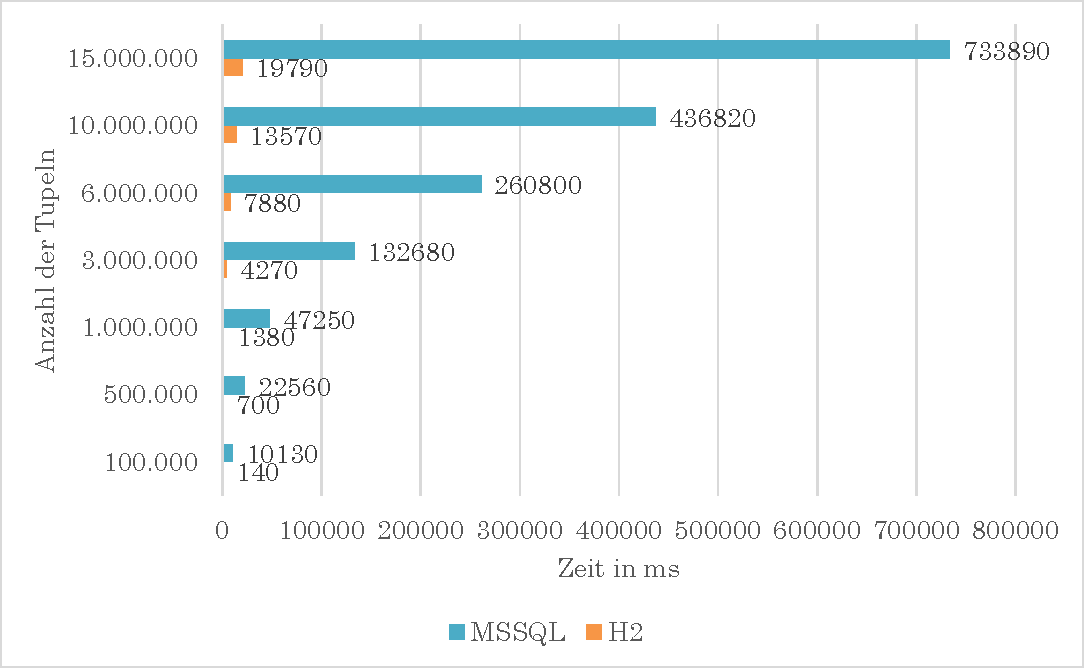
\includegraphics[width=0.49\textwidth]{charts/select.pdf}}\hfill
\subfigure[Vergleich anhand Update-Performance]{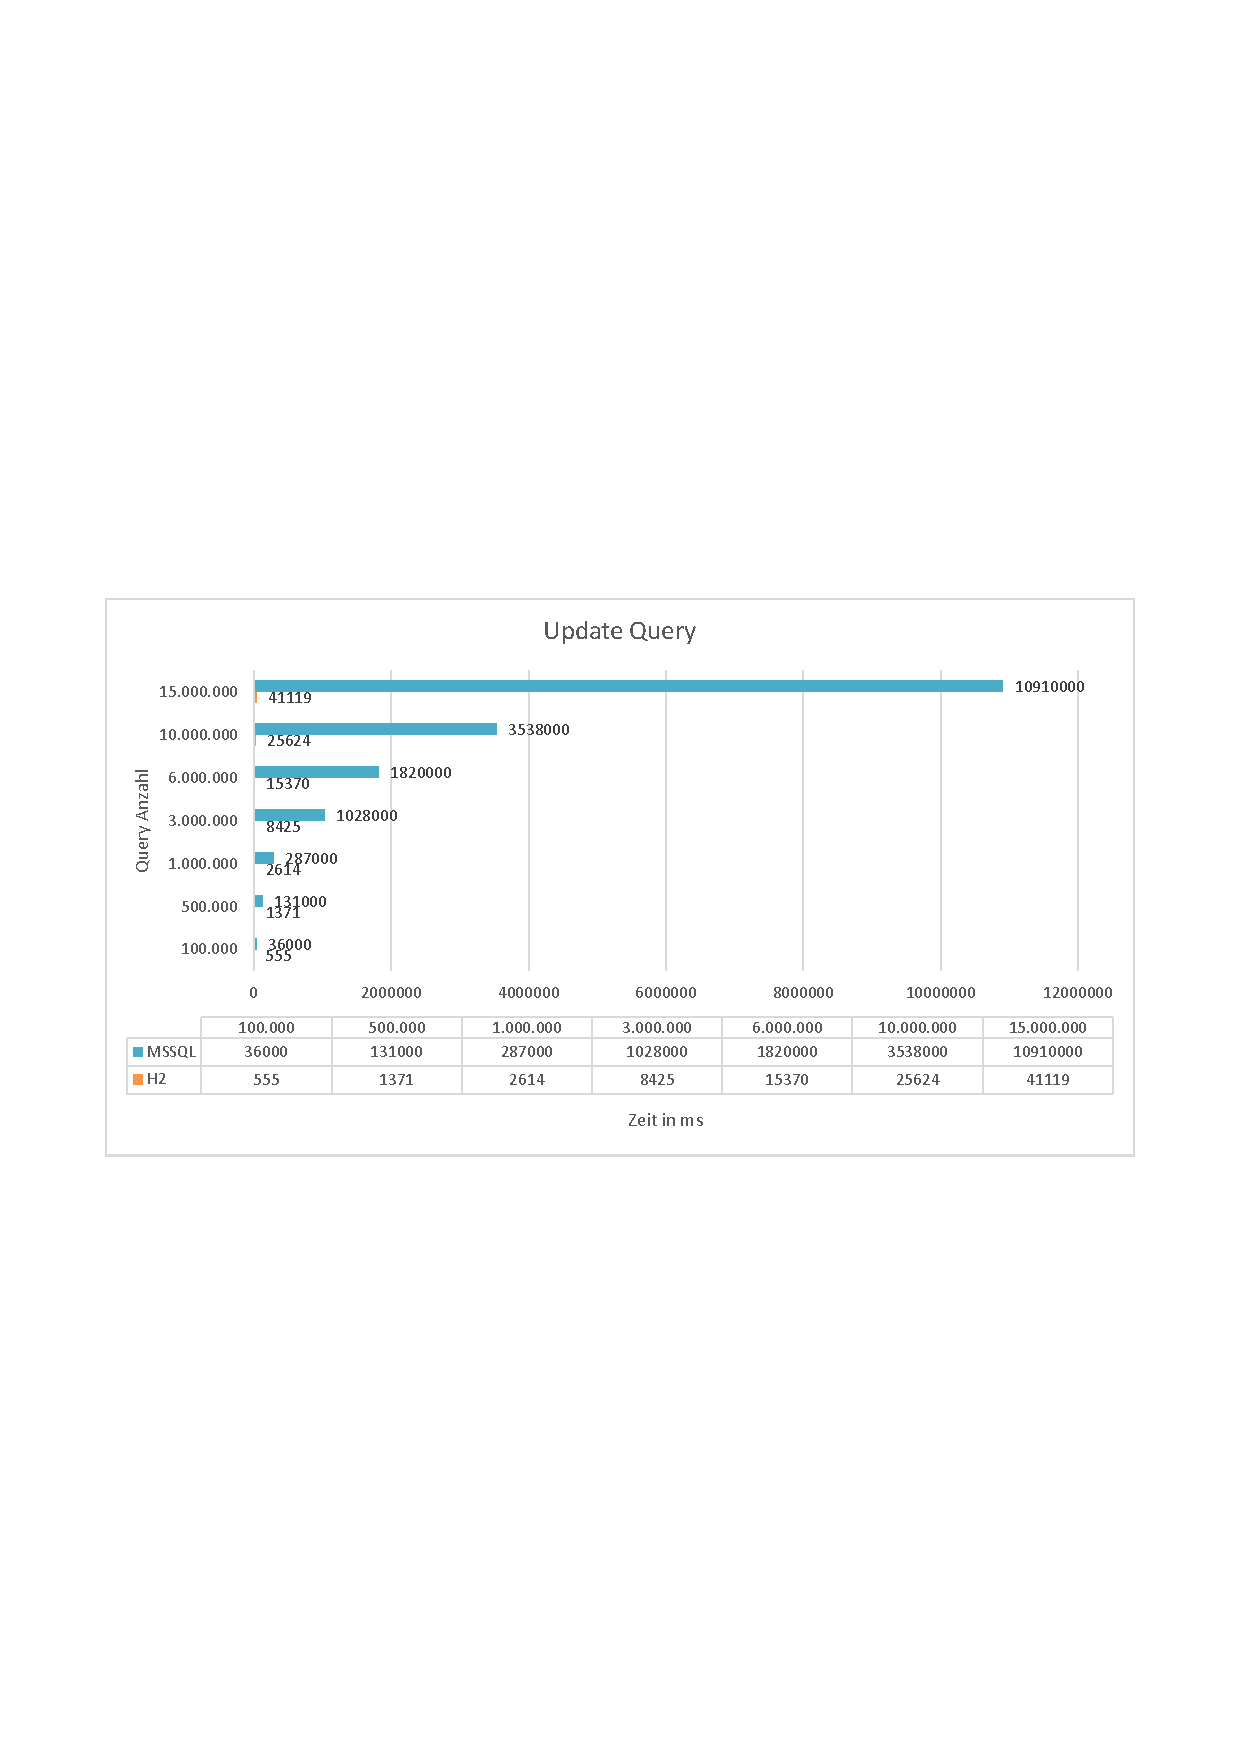
\includegraphics[width=0.49\textwidth]{charts/update.pdf}}\hfill
\subfigure[Vergleich anhand Insert-Performance]{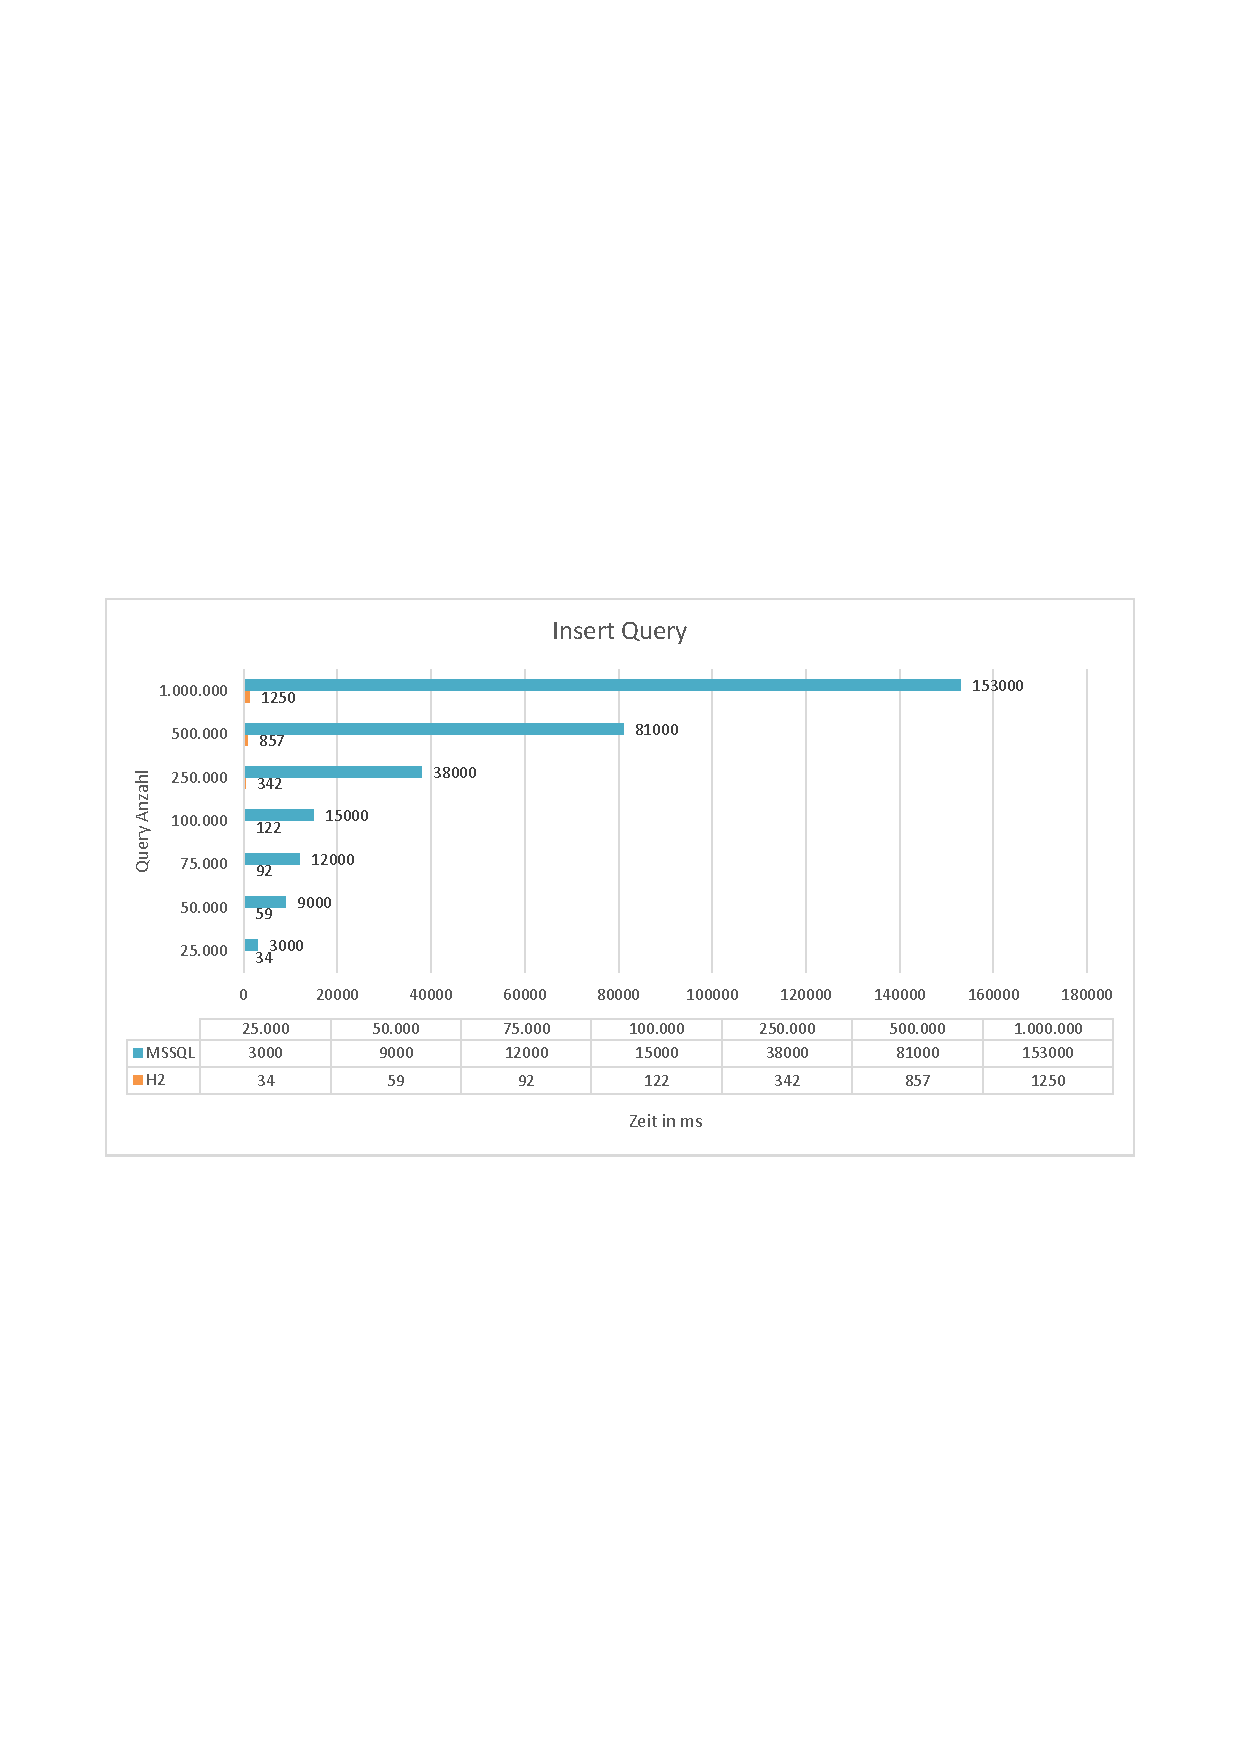
\includegraphics[width=0.5\textwidth]{charts/insert.pdf}}
\caption{Abfragegeschwindigkeit Vergleich}
\label{ergebniss_vergleich}
\end{figure}


%% ===========================
\section{Handlungsempfehlungen}
%% ===========================

...
